
%(BEGIN_QUESTION)
% Copyright 2014, Tony R. Kuphaldt, released under the Creative Commons Attribution License (v 1.0)
% This means you may do almost anything with this work of mine, so long as you give me proper credit

Suppose a Rosemount model 3244MV (FOUNDATION Fieldbus) transmitter is used as a voltage sensor for a strain gauge bridge circuit, the transmitter configured to sense DC millivolt input and report the amount of strain in pounds of force.  The bridge circuit and strain gauge are designed to output 1.5 millivolts of signal per pound of applied force:

$$\includegraphics[width=15.5cm]{i00962x01.eps}$$

Determine the proper {\tt XD\_Scale}, {\tt OUT\_Scale}, and {\tt L\_Type} parameter values to make the transmitter functional over the strain gauge's range of 0 to 35 pounds.

\underbar{file i00962}
%(END_QUESTION)





%(BEGIN_ANSWER)

{\tt L\_Type} = Indirect

\vskip 10pt

{\tt XD\_Scale} = 0 to 52.5 mV

\vskip 10pt

{\tt OUT\_Scale} = 0 to 35 pounds

%(END_ANSWER)





%(BEGIN_NOTES)

{\bf This question is intended for exams only and not worksheets!}.

%(END_NOTES)


